\documentclass[12pt]{article}
\usepackage{makecell}
\usepackage{hyphenat}
\usepackage[utf8]{vietnam}
\usepackage[vietnamese=nohyphenation]{hyphsubst}
\usepackage[vietnamese]{babel}
\usepackage[table,dvipsnames]{xcolor} % Required for row coloring
\usepackage{booktabs} % Required for nicer horizontal lines
\usepackage{ragged2e}
\usepackage{caption}
\usepackage{subcaption}
\usepackage{float}
\usepackage{amsmath,amssymb,amsfonts}
\usepackage{graphicx}
\usepackage{adjustbox}
\usepackage{multicol}
\usepackage[inline,shortlabels]{enumitem}
\usepackage{setspace}
\usepackage{longtable}
\usepackage{bm} 
\usepackage[inkscapelatex=false]{svg}
\usepackage{titling}
\usepackage{tabularx}
\usepackage[T1]{fontenc}
\usepackage{lmodern,mathrsfs}
% \usepackage[draft]{hyperref}
\usepackage{hyperref}
\usepackage{xparse}
\usepackage{fontawesome5}
\usepackage[most]{tcolorbox}
\usepackage{tikz}
\usepackage[framemethod=TikZ]{mdframed}
\usetikzlibrary{matrix, fit, shadows, positioning, arrows.meta, calc, shapes.geometric, backgrounds, shapes.symbols}
\usepackage{paracol}
\usepackage{bbm}
\usepackage{pgfplots}
\usepackage{siunitx}
\usepackage{multirow}
%  biblatex (thay cho IEEEtran.bst) ------------------------------------
\usepackage[
    backend=bibtex,
    style=ieee,
    citestyle=numeric-comp,
    maxnames=1,     % chỉ hiển thị 1 tên tác giả, phần còn lại thành ``et al."
    minnames=1,
    uniquelist=false,
    hyperref=false
]{biblatex}
\usepackage{forest}
% \addbibresource{references.bib} % bỏ trống vì tài liệu này chưa dùng citation
\DefineBibliographyStrings{english}{
  andothers = {et\addabbrvspace al\adddot}
}
\AtBeginBibliography{\selectlanguage{english}}

% -----------------------------------------------------------------
\AtBeginDocument{\renewcommand\refname{}}

\usepackage[toc,page]{appendix}
\renewcommand{\appendixtocname}{Phụ lục}      
\renewcommand{\appendixpagename}{Phụ lục}

\usepackage{xurl}
\setlength{\headheight}{14.5pt}
\setlength{\topmargin}{-.5in} \setlength{\textheight}{9.25in}
\setlength{\oddsidemargin}{-0.1in} \setlength{\textwidth}{6.8in}

\usepackage{tocloft}
\renewcommand{\cfttoctitlefont}{\Huge\bfseries}
\setlength{\cftaftertoctitleskip}{2em}
\setlength{\cftbeforesubsecskip}{7pt} % giãn cách subitem mục lục
\renewcommand{\cftsecleader}{\cftdotfill{\cftdotsep}}
\setlength{\cftsecnumwidth}{3em}
\renewcommand{\cftsecaftersnum}{\quad}
\renewcommand{\cftsubsecleader}{\cftdotfill{\cftdotsep}}
\setlength{\cftsubsecnumwidth}{4em}
\renewcommand{\cftsubsecaftersnum}{\quad}
\renewcommand{\cftsubsubsecleader}{\cftdotfill{\cftdotsep}}
\setlength   {\cftsubsubsecnumwidth}{5em}  
\renewcommand{\cftsubsubsecaftersnum}{\quad}

\PassOptionsToPackage{vietnamese.licr}{babel}
\usepackage{../../latex/styles/vipythonhighlight}
\usepackage{../../latex/styles/tvietlistings}
\newcounter{mycounter}
\newcommand\showmycounter{\stepcounter{mycounter}\themycounter}
\usepackage{lipsum}
\newcommand\showlips{\stepcounter{mycounter}\lipsum[\value{mycounter}]}

%--------------------------------------------------------------------
\usepackage{framed}
\usepackage{fancyhdr}
\usepackage{upquote}
\usepackage{listings}	 

\usepackage[toc, nonumberlist, style=super]{glossaries}
\makenoidxglossaries

\newglossarystyle{clean3col}{%
    % 1) Table layout: 3 columns
    \renewenvironment{theglossary}%
    {%
      \begin{longtable}{@{}
        >{\setlength{\parindent}{0pt}\RaggedRight\arraybackslash}p{0.2\linewidth}
        >{\setlength{\parindent}{0pt}\RaggedRight\arraybackslash}p{0.23\linewidth}
        >{\setlength{\parindent}{0pt}\RaggedRight\arraybackslash}p{0.52\linewidth}
      @{}}%
    }%
    {\end{longtable}}%

    % 2) Header row
    \renewcommand{\glossaryheader}{%
        \bfseries Thuật ngữ &
        \bfseries Tạm dịch &
        \bfseries Mô tả \\
        \midrule
        \endhead
    }%

    % 3) Each entry row
    \renewcommand{\glossentry}[2]{%
        \itshape \glstarget{##1}{\glossentryname{##1}} &
        \glsentryuseri{##1} &
        \glossentrydesc{##1} \\
        \addlinespace[6pt]
    }%
}


% Color --------------------------------------------------------------------
\usepackage{epigraph}
\usepackage{titlesec}

\definecolor{codebackground}{RGB}{250, 250, 250}
\definecolor{codecomment}{RGB}{34, 139, 34}
\definecolor{codekeyword}{RGB}{0, 0, 255}
\definecolor{codestring}{RGB}{255, 0, 0}
\definecolor{codeidentifier}{RGB}{0, 0, 0}
\definecolor{codelinenumbers}{RGB}{90, 90, 90}

\definecolor{codegreen}{rgb}{0,0.6,0}
\definecolor{codegray}{rgb}{0.5,0.5,0.5}
\definecolor{codepurple}{rgb}{0.58,0,0.82}
\definecolor{backcolour}{rgb}{0.95,0.95,0.92}

\definecolor{aivnGreen}{RGB}{52,79,30}  
\definecolor{aivnCodeOutputColor}{RGB}{11,83,148}  
\definecolor{captiongray}{gray}{0.15} 
\definecolor{captionbg}{RGB}{250,250,250}

\definecolor{foldercolor}{RGB}{0, 102, 204}
\definecolor{filecolor}{RGB}{104, 104, 104}
\definecolor{scriptcolor}{RGB}{180, 50, 50}
\definecolor{pythoncolor}{RGB}{0, 128, 128}

% --- Extra Brand colors for the table ---
\definecolor{brandIndigo}{HTML}{333D91} 
\definecolor{rowLavender}{HTML}{EEECFA}
\setlength{\parskip}{0.3em}

% Table
\newtcolorbox{captionbelowboxaivn}{
    colback=aivnGreen,
    colframe=aivnGreen,
    boxrule=0pt,
    arc=4pt,
    left=4pt,
    right=4pt,
    top=2pt,
    bottom=2pt,
    width=\linewidth,
    boxsep=4pt,
    halign=center,
    % fontupper=\bfseries\color{white}
    fontupper=\color{white}
}

% Figure
\newtcolorbox{figurecardcaptionaivn}{
  colback=aivnGreen,        % Màu nền (background color)
  colframe=aivnGreen,       % Màu viền box (border color)
  boxrule=0pt,              % Độ dày viền box (0pt = không viền)
  arc=2pt,                  % Độ bo góc (2pt là bo nhẹ, tăng để bo tròn hơn)
  top=3pt,                  % Padding phía trên nội dung
  bottom=3pt,               % Padding phía dưới nội dung
  left=10pt,                % Padding bên trái
  right=10pt,               % Padding bên phải
  width=\linewidth,         % Chiều rộng bằng toàn bộ dòng
  fontupper=\small\fontsize{11pt}{13pt}\selectfont\color{white} 
}

% Tạo counter riêng
\newcounter{hinh}
% Định nghĩa macro caption Hình
\newcommand{\capfig}[1]{%
  \refstepcounter{hinh}%
  % \textbf{Hình~\thehinh:}~#1
    Hình~\thehinh:~#1
}

\newtcolorbox{figurecaptionmodern}{
  colback=captionbg,
  colframe=aivnGreen,
  boxrule=1.5pt,
  bottomrule=2pt,  
  toptitle=0pt,
  bottomtitle=0pt,
  left=6pt,
  right=6pt,
  top=4pt,
  bottom=2pt,
  width=\linewidth,
  fontupper=\small\fontsize{11pt}{13pt}\selectfont\color{black},
  halign=center
}

% Code Block -----------------------------------------------------------------
\newtcolorbox{aivncodebox}[1][]{%
  enhanced,
  colback=gray!10,
  colframe=aivnGreen,
  coltitle=white,
  colbacktitle=aivnGreen,
  title=#1,
  fonttitle=\bfseries\sffamily,
  listing only,
  breakable,
  listing engine=listings,
  listing options={
    language=Python,
    basicstyle=\ttfamily\footnotesize,
    commentstyle=\color{ForestGreen},
    keywordstyle=\color{blue},
    stringstyle=\color{red!70!black},
    numbers=left, upquote=true,
    numberstyle=\tiny\color{gray},
    numbersep=5pt,
    breaklines=true,
    showstringspaces=false,
    xleftmargin=1.5em,
    framexleftmargin=1.5em
  }
}

% Code Output Block -----------------------------------------------------------------
\newtcolorbox{aivnCodeOutput}[1][]{%
  enhanced,
  colback=gray!10,
  colframe=aivnCodeOutputColor,
  coltitle=white,
  colbacktitle=aivnCodeOutputColor,
  title=#1,
  fonttitle=\bfseries\sffamily,
  listing only,
  breakable,
  listing engine=listings,
  listing options={
    language=Python,
    basicstyle=\ttfamily\footnotesize,
    commentstyle=\color{ForestGreen},
    keywordstyle=\color{blue},
    stringstyle=\color{red!70!black},
    numbers=left,
    numberstyle=\tiny\color{gray},
    numbersep=5pt,
    breaklines=true,
    showstringspaces=false,
    xleftmargin=1.5em,
    framexleftmargin=1.5em
  }
}

% Last argument allows more tcolorbox options to be added

% --- SQL code box ------------------------------------------------------------
\lstdefinestyle{sqlstyle}{
    backgroundcolor=\color{codebackground},
    keywordstyle=\color{blue}\bfseries,
    stringstyle=\color{red!70!black},
    commentstyle=\color{ForestGreen}\itshape,
    basicstyle=\ttfamily\footnotesize,
    columns=fullflexible,
    keepspaces=true,
    numbers=left,
    numberstyle=\tiny\color{gray},
    numbersep=5pt,
    breaklines=true,
    showstringspaces=false,
    upquote=true,
    xleftmargin=1.5em,
    framexleftmargin=1.5em
}

\newtcblisting{aivnsqlbox}[1][]{%
  enhanced,
  colback=gray!10,
  colframe=aivnGreen,
  coltitle=white,
  colbacktitle=aivnGreen,
  title=#1,
  fonttitle=\bfseries\sffamily,
  listing only,
  breakable,
  listing engine=listings,
  listing options={language=SQL, style=sqlstyle}
}

% --- Plain text / config (YAML, Jinja) code box ------------------------------
\lstdefinestyle{plainstyle}{
    backgroundcolor=\color{codebackground},
    basicstyle=\ttfamily\footnotesize,
    columns=fullflexible,
    keepspaces=true,
    numbers=left,
    numberstyle=\tiny\color{gray},
    numbersep=5pt,
    breaklines=true,
    showstringspaces=false,
    upquote=true,
    xleftmargin=1.5em,
    framexleftmargin=1.5em
}

\newtcblisting{aivnplainbox}[1][]{%
  enhanced,
  colback=gray!10,
  colframe=aivnCodeOutputColor,
  coltitle=white,
  colbacktitle=aivnCodeOutputColor,
  title=#1,
  fonttitle=\bfseries\sffamily,
  listing only,
  breakable,
  listing engine=listings,
  listing options={language={}, style=plainstyle}
}

% --- Placeholder cho sơ đồ cần vẽ sau ----------------------------------------
\newcommand{\diagramplaceholder}[2][5.5cm]{%
  \begin{center}
  \begin{tcolorbox}[enhanced, breakable,
      colback=gray!4, colframe=gray!60, boxrule=0.8pt, arc=4pt,
      width=\linewidth, height=#2, valign=center, halign=center]
    {\color{gray}\sffamily\faImage\hspace{1em}\textbf{[PLACEHOLDER --- Sơ đồ]}}\\[8pt]
    {\color{gray}\sffamily\itshape #1}
  \end{tcolorbox}
  \end{center}
}

% --- Guideline/Tip box ---
\newtcolorbox{guidelinebox}[2][]{
    enhanced, colback=yellow!10!white, colframe=orange!90!black, boxrule=1pt, arc=4pt,
    fonttitle=\bfseries, attach boxed title to top left={yshift=-2mm, xshift=3mm},
    colbacktitle=orange!90!black, coltitle=white,
    title=\faLightbulb\hspace{1mm} #2, #1
}

\newtcolorbox{notebox}[1][]{
  enhanced,  colback=yellow!10, colframe=orange!80, boxrule=1pt, 
  arc=4pt, fontupper=\small, attach boxed title to top left={yshift=-2mm, xshift=3mm},
  colbacktitle=orange!80,  coltitle=white, fonttitle=\bfseries,  
  title=\faInfoCircle~\textbf{Lưu ý},  #1
}

\newtcolorbox{infobox}[1]{%
    enhanced, 
    breakable, 
    colback=green!3, 
    colframe=green!3, 
    arc=5pt,
    borderline west={3pt}{0pt}{aivnGreen},
    attach boxed title to top left={ 
        yshift*=-\tcboxedtitleheight/2, 
        xshift=-0.1em 
    },
    colbacktitle=aivnGreen, %
    coltitle=white, 
    fonttitle=\bfseries, 
    boxed title style={ 
        arc=4pt, 
        top=2pt, 
        bottom=2pt,
        left=8pt,
        right=8pt,
    },
    title={\faInfoCircle\quad #1}
}
\newtcolorbox{examplebox}[1]{%
    enhanced,
    breakable,
    colback=brandIndigo!5,      
    colframe=brandIndigo!5,     
    arc=5pt,
    borderline west={3pt}{0pt}{brandIndigo}, 
    attach boxed title to top left={
        yshift*=-\tcboxedtitleheight/2,
        xshift=-0.1em
    },
    colbacktitle=brandIndigo,   
    coltitle=white,
    fonttitle=\bfseries,
    boxed title style={
        arc=4pt,
        top=2pt,
        bottom=2pt,
        left=8pt,
        right=8pt,
    },
    title={\faLightbulb\quad #1} 
}
% Prompt Block ---------------------------------------------------------------
\definecolor{promptBlue}{HTML}{2F5D8C}
\definecolor{promptBg}{HTML}{F6F9FC}
\definecolor{promptBorder}{HTML}{B7C9DC}

% Dùng cho prompt đã viết theo cú pháp LaTeX bình thường
\newtcolorbox{promptbox}[1][Prompt]{%
    enhanced,
    breakable,
    colback=promptBg,
    colframe=promptBorder,
    coltitle=white,
    colbacktitle=promptBlue,
    fonttitle=\bfseries\sffamily,
    title={#1},
    boxrule=0.8pt,
    arc=4pt,
    left=8pt,
    right=8pt,
    top=2pt,
    bottom=1pt,
    before skip=8pt,
    after skip=8pt,
    borderline west={3pt}{0pt}{promptBlue},
    fontupper=\small\sffamily,
}

% Dùng cho prompt raw: giữ nguyên xuống dòng, không highlight keyword
\newtcblisting{promptboxraw}[1][Prompt]{%
    enhanced,
    breakable,
    listing only,
    listing engine=listings,
    colback=promptBg,
    colframe=promptBorder,
    coltitle=white,
    colbacktitle=promptBlue,
    fonttitle=\bfseries\sffamily,
    title={#1},
    boxrule=0.8pt,
    arc=4pt,
    left=8pt,
    right=8pt,
    top=-4pt,
    bottom=-4pt,
    before skip=4pt,
    after skip=4pt,
    borderline west={3pt}{0pt}{promptBlue},
    listing options={
        language={},
        basicstyle=\small\ttfamily,
        columns=fullflexible,
        keepspaces=true,
        breaklines=true,
        showstringspaces=false,
        numbers=none,
        frame=none,
        keywordstyle=\color{black},
        commentstyle=\color{black},
        stringstyle=\color{black},
        identifierstyle=\color{black}
    }
}


%--------------------------------------------------------------------
\lstdefinestyle{mystyle}{
    backgroundcolor=\color{codebackground},
    commentstyle=\color{codecomment},
    keywordstyle=\color{codekeyword},
    stringstyle=\color{codestring},
    identifierstyle=\color{codeidentifier},
    basicstyle=\ttfamily\footnotesize,
    breakatwhitespace=false,
    breaklines=true,
    captionpos=b,
    keepspaces=true,
    numbers=left,
    numberstyle=\tiny\color{codelinenumbers}, 
    numbersep=5pt,
    showspaces=false,
    showstringspaces=false,
    showtabs=false,
    tabsize=2
}

\lstset{style=mystyle}

\hypersetup{
    colorlinks=true,
    linkcolor=black,
    filecolor=magenta,    
    citecolor=green,
    urlcolor=blue,
    pdftitle={Tài liệu đọc: Slowly Changing Dimension (SCD Type 2)},
    pdfpagemode=FullScreen,
}

%--------------------------------------------------------------------
\newcounter{choice}
\renewcommand\thechoice{($\alph{choice}$)}
\newcommand\choicelabel{\thechoice}

%--------------------------------------------------------------------
\newenvironment{choices}%
  {\list{\choicelabel}%
     {\usecounter{choice}\def\makelabel##1{\hss\llap{##1}}%
       \settowidth{\leftmargin}{W.\hskip\labelsep\hskip 0 em}%
       \def\choice{%
         \item
       } % choice
       \labelwidth\leftmargin\advance\labelwidth-\labelsep
       \topsep=0pt
       \partopsep=0pt
     }%
  }%
  {\endlist}
  
%--------------------------------------------------------------------
\def\CChoice{%
      \choice
      \addanswer{\theenumi}{\thechoice}%
    }
    \let\CChoice\CChoice
%    \par % Uncomment this to have choices always start a new line
   % \let\par\@empty
    % If we're continuing the textbf containing the question,
    % then leave a bit of space before the first choice:
    \ifvmode\else\enskip\fi
    \ignorespaces
  %
  {}
\makeatother
\newbox\allanswers
\setbox\allanswers=\hbox{}
\newcommand{\addanswer}[2]{%
  \global\setbox\allanswers=\hbox{\unhbox\allanswers \quad #1.~#2}%
}
\newcommand{\showanswers}{%
  \vfill
  \begin{center}
    Answers
  \end{center}
  \unhbox\allanswers
}

\makeatletter
\newenvironment{multichoices}[1][1]{%
\begin{multicols}{#1}}{%
\end{multicols}}
\makeatother

\pagestyle{fancy}

\DeclareMathOperator*{\argmax}{arg\,max}
\DeclareMathOperator*{\argmin}{arg\,min}
\DeclareMathOperator{\E}{\mathbb{E}}

% Outline --------------------------------------------------------------------
% Section numbering ----------------------------------------------------------
\renewcommand{\thesection}{\Roman{section}.} 
\renewcommand{\thesubsection}{\thesection\arabic{subsection}.}
\renewcommand{\thesubsubsection}{\thesubsection\arabic{subsubsection}.}

% Paper-like section title sizes --------------------------------------------
% Title paper: 17pt
% Section should be clearly smaller than title but still prominent.
\titleformat{\section}
  {\normalfont\fontsize{16pt}{20pt}\selectfont\bfseries}
  {\thesection}
  {0.85em}
  {}

\titleformat{\subsection}
  {\normalfont\fontsize{14pt}{16pt}\selectfont\bfseries}
  {\thesubsection}
  {0.75em}
  {}

\titleformat{\subsubsection}
  {\normalfont\fontsize{12pt}{15pt}\selectfont\bfseries}
  {\thesubsubsection}
  {0.65em}
  {}

% Paper-like compact spacing -------------------------------------------------
\titlespacing*{\section}
  {0pt}
  {1.25em plus 0.2em minus 0.1em}
  {0.65em plus 0.1em minus 0.1em}

\titlespacing*{\subsection}
  {0pt}
  {1.0em plus 0.2em minus 0.1em}
  {0.45em plus 0.1em minus 0.1em}

\titlespacing*{\subsubsection}
  {0pt}
  {0.85em plus 0.15em minus 0.1em}
  {0.35em plus 0.1em minus 0.1em}


% Logo + Title ---------------------------------------------------------------

\setlength{\droptitle}{-7em}

% Title horizontal rule
\newcommand{\TitleRule}{%
  \rule{0.90\textwidth}{0.6pt}
}

% Chiều cao vùng title giữa 2 rule
\newlength{\TitleBlockHeight}
\setlength{\TitleBlockHeight}{2.6cm}

\pretitle{%
  

  % Logo row
  \begin{tabular}{@{}c@{\hspace{1.0em}}c@{\hspace{1.0em}}c@{}}
    \raisebox{-0.35\height}{
\includegraphics[height=2.0cm]{../../shared/figures/aio2026_logo.pdf}}    
  \end{tabular}

  %\vspace{0.2em}

\begin{center}
  \TitleRule
  \par\nointerlineskip
}

\title{%
  \parbox[c][\TitleBlockHeight][c]{0.90\textwidth}{%
    \centering
    {\fontsize{17pt}{21pt}\selectfont\bfseries Tài liệu đọc: Slowly Changing Dimension (SCD Type 2)\\[3pt]
     \fontsize{13pt}{16pt}\selectfont Theo dõi lịch sử thay đổi dữ liệu trong Data Mart}
  }%
}

\posttitle{%
  \par\nointerlineskip
  \TitleRule
  \end{center}
}

\preauthor{%
  \begin{center}
  \fontsize{11pt}{13pt}\selectfont
}

\author{%
  \textbf{name\_1}
  \hspace{2.8em}
  \textbf{name\_2}\\
  \vspace{1em}
  \textbf{Proofreading: }
}

\postauthor{%
  \par
  \end{center}
}

\date{}
% Header --------------------------------------------------------------------
\pagestyle{fancy}
\fancyhf{}
\lhead{\href{https://www.facebook.com/aivietnam.edu.vn}{\textcolor{aivnGreen}{\bfseries AI VIET NAM (AIO2026)}}}
\rhead{\href{https://aivietnam.edu.vn/}{\textcolor{aivnGreen}{\bfseries aivietnam.edu.vn}}}
\fancyfoot[r]{\textcolor{aivnGreen}{\bfseries Trang \thepage}}
\fancyfoot[l]{%
  \href{https://zalo.me/84911118758}{%
    \textcolor{aivnGreen}{\bfseries SĐT/Zalo: 0911118758 (Dr. Hồng Phúc)}%
  }%
}
\renewcommand{\headrulewidth}{1.0pt}
\renewcommand{\headrule}{{\color{aivnGreen}\hrule width\headwidth height\headrulewidth \vskip-\headrulewidth}}

\renewcommand{\footrulewidth}{1.0pt}
\renewcommand{\footrule}{{\color{aivnGreen}\hrule width\headwidth height\footrulewidth \vskip-\footrulewidth}}


\fancypagestyle{firstpage}{
    \fancyhf{}
    \fancyfoot[r]{\textcolor{aivnGreen}{\bfseries Trang \thepage}}
    \fancyfoot[l]{%
      \href{https://zalo.me/84911118758}{%
        \textcolor{aivnGreen}{\bfseries SĐT/Zalo: 0911118758 (Dr. Hồng Phúc)}%
      }%
    }
    \renewcommand{\headrulewidth}{0pt}
    \renewcommand{\footrulewidth}{1.0pt}
    \renewcommand{\footrule}{%
        {\color{aivnGreen}\hrule width\headwidth height\footrulewidth}
    }
}


\begin{document}
\maketitle
\thispagestyle{firstpage}
\vspace{-3em}

% =============================================================
\section{Lời mở đầu}

Trong tài liệu trước, chúng ta đã xây dựng được \texttt{mart\_customer\_360} --- một bảng khách hàng với các chỉ số LTV, Segment và Tier. Nhưng hãy tưởng tượng tình huống sau, một trong những câu hỏi muôn thuở thực tế nhất của Data Warehousing:

\begin{examplebox}{Tình huống báo cáo lệch}
\textit{``Tháng 12, khách hàng Phạm Thị B đạt đủ điều kiện lên hạng \textbf{Platinum}. Nhưng khi rà soát doanh thu quý IV để tính thưởng, trưởng phòng Sales khẳng định: 'Khách B là khách Platinum, doanh thu nhóm Platinum phải là 2 tỷ' --- trong khi báo cáo của anh chốt doanh thu nhóm Platinum Quý IV chỉ đạt 1.2 tỷ. Vậy ai đúng? Đâu là số đúng?''}
\end{examplebox}

\begin{figure}[H]
  \centering
  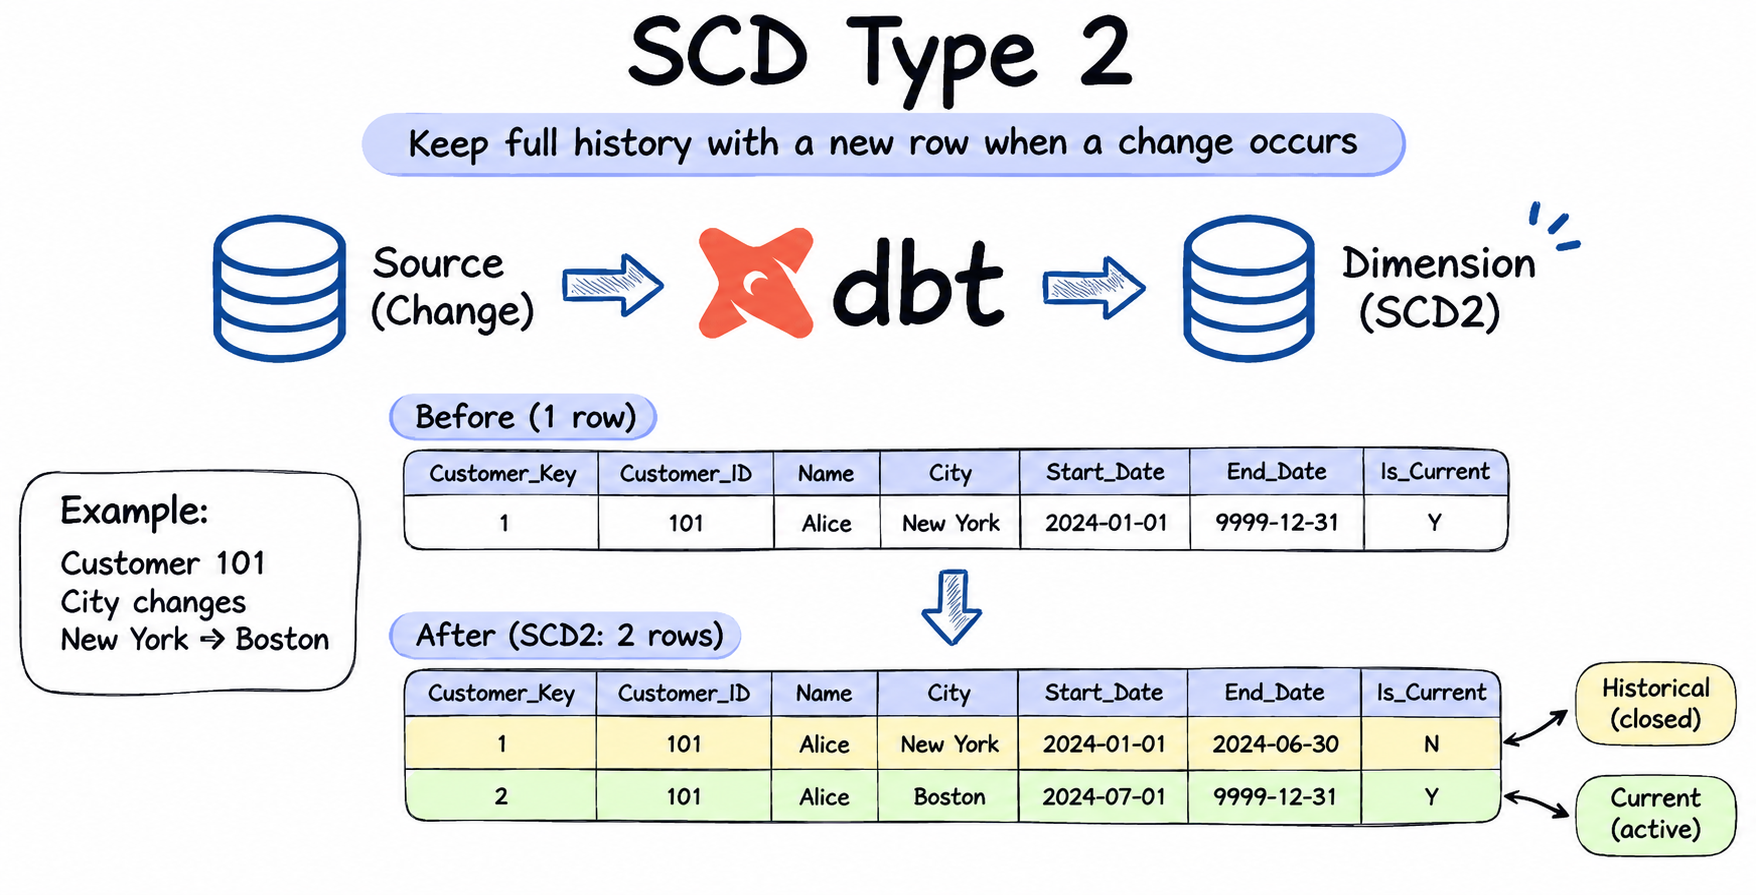
\includegraphics[width=\textwidth]{figures/SCD Type 2 History Flow Infographic.png}
  \caption{Sơ đồ dòng lịch sử của SCD Type 2.}
  \label{fig:scd2-history-flow}
\end{figure}

Cả hai đều đúng, nhưng đang nói về \textbf{hai mốc thời gian khác nhau} của cùng một thực thể:
\begin{itemize}
    \item Trưởng phòng Sales đang nói về \textbf{hiện tại}: hôm nay Phạm Thị B là Platinum.
    \item Báo cáo Quý IV đang nói về \textbf{quá khứ}: trong tháng 10, 11 và phần lớn tháng 12, khách B vẫn là khách hạng \textbf{Gold} trước khi lên hạng.
\end{itemize}

Bài toán này không nằm ở dashboard, mà nằm ở cách lưu trữ chiều (dimension) phía dưới. Trong tài liệu trước, chúng ta đối xử với \texttt{dim\_customer} như một bảng ``thuần khiết'' --- nơi mỗi khách hàng chỉ có \textbf{một dòng duy nhất}, đóng vai trò nguồn chân lý duy nhất (Single Source of Truth). Nhưng khi thông tin khách hàng thay đổi theo thời gian, nếu ta vẫn \texttt{UPDATE} ``một dòng duy nhất'' đó (overwrite in-place giống hệt hệ thống OLTP), sẽ có một hệ quả nặng nề:

\begin{notebox}
\textbf{Báo cáo cho cùng một kỳ lịch sử sẽ cho ra kết quả khác nhau tùy thời điểm bạn chạy truy vấn.} Nhóm Platinum Quý IV hôm nay là 1.2 tỷ, nhưng chạy lại báo cáo này vào tháng sau có thể thành 1.6 tỷ --- Single Source of Truth vỡ vụng ngay tại chỗ. Trong kho dữ liệu, \texttt{UPDATE} in-place đồng nghĩa với việc \textbf{phá hủy lịch sử báo cáo} (breaking historical reporting).
\end{notebox}

Tài liệu này được biên soạn nhằm giúp bạn:
\begin{enumerate}
    \item Nhận diện được nhóm dữ liệu nào \textit{thay đổi chậm} (slowly changing), và tại sao \texttt{UPDATE} in-place --- điều hệ OLTP vẫn làm mỗi ngày --- lại là sai lầm nghiêm trọng trong kho dữ liệu.
    \item Nắm vững bản đồ họ giải pháp SCD từ Type 0 đến Type 6, và lý giải vì sao \textbf{Type 2} (tạo dòng mới kèm đánh dấu khoảng hiệu lực) lại trở thành lựa chọn chuẩn mực của ngành.
    \item Thiết kế đúng cấu trúc bảng SCD Type 2 theo chuẩn Kimball: surrogate key, khoảng hiệu lực (\texttt{valid\_from} / \texttt{valid\_to}), cờ hiện tại (\texttt{is\_current}).
    \item Hiện thực hóa SCD Type 2 một cách tự động hóa hoàn chỉnh qua \textbf{dbt snapshot}, thay vì viết SQL merge thủ công mỗi lần pipeline chạy.
    \item Đánh giá các điểm đánh đổi: khi nào nên track toàn bộ cột, khi nào chỉ track vài cột quan trọng, và khi nào thì SCD Type 2 là giải pháp ``giết gà dùng dao mổ trâu'' --- phức tạp hóa không cần thiết.
\end{enumerate}

% =============================================================

\section{Outline của tài liệu}

Để có cái nhìn tổng quan trước khi đi vào chi tiết, tài liệu được tổ chức thành 6 phần như sau:

% -------------------------------------------------------------
\noindent
\begin{longtable}{@{}>{\RaggedRight\arraybackslash}p{3.1cm}>{\RaggedRight\arraybackslash}p{8.3cm}>{\RaggedRight\arraybackslash}p{4.3cm}@{}}
\rowcolor{rowLavender}
\textbf{Phần} & \textbf{Nội dung} & \textbf{Vấn đề cốt lõi} \\
\addlinespace[3pt]
\endhead

\textbf{1. Bài toán dữ liệu ``sống'' theo thời gian} 
& Dimension trong kho dữ liệu không phải dữ liệu tĩnh: khách hàng đổi địa chỉ, đổi hạng thành viên; sản phẩm đổi giá, đổi danh mục; nhân viên đổi phòng ban. Về bản chất, vấn đề sẽ là: dòng nào trong bảng \texttt{dim\_customer} là ``bản sự thật'' tại một thời điểm bất kỳ?
& Không thể \texttt{UPDATE} in-place mà không phá hủy lịch sử báo cáo \\
\addlinespace[6pt]

\textbf{2. Phân loại các chiến lược SCD}
& So sánh toàn bộ họ giải pháp SCD: Type 0, Type 1, Type 2, Type 3, Type 4 (mini-dimension), Type 6 (hybrid). Tại sao Type 2 trở thành chuẩn công nghiệp.
& Lựa chọn chiến lược phù hợp theo yêu cầu nghiệp vụ \\
\addlinespace[6pt]

\textbf{3. Thiết kế cấu trúc bảng SCD Type 2}
& Thiết kế cột hiệu lực (\texttt{valid\_from}, \texttt{valid\_to}), cờ hiện tại (\texttt{is\_current}), surrogate key, và biến thể đánh số phiên bản (version number). Điểm mấu chốt: một thực thể nghiệp vụ (business key) sẽ có \textbf{nhiều dòng} tương ứng nhiều giai đoạn.
& Cấu trúc dữ liệu đúng chuẩn Kimball \\
\addlinespace[6pt]

\textbf{4. Cơ chế phát hiện thay đổi và xử lý dữ liệu}
& Logic phát hiện thay đổi (so sánh giá trị, \texttt{CHECKSUM}, hash của các cột cần track), xử lý snapshot trùng lặp (không tạo version giả không cần thiết), xử lý back-dating (thay đổi có thời điểm hiệu lực lùi về giữa lịch sử).
& Pipeline chạy hàng ngày vẫn phải đúng \\
\addlinespace[6pt]

\textbf{5. Hiện thực hóa SCD Type 2 bằng dbt}
& Cơ chế \texttt{dbt snapshot} với \texttt{check strategy} và \texttt{timestamp strategy}, biến \texttt{invalidate\_hard\_deletes}, và cách truy vấn ``bản dữ liệu tại thời điểm T'' (point-in-time query) kết hợp với Fact table.
& Vận hành SCD2 bằng code, không viết SQL merge thủ công \\
\addlinespace[6pt]

\textbf{6. Trade-offs và thảo luận thực tế}
& Chi phí lưu trữ tăng theo số version, ảnh hưởng hiệu năng JOIN (fan-out khi join sai điều kiện hiệu lực), chiến lược chọn cột track (ít cột quan trọng vs. toàn bộ), và khi nào thì SCD Type 2 là \textbf{overkill}.
& Cân bằng giữa lịch sử đầy đủ và chi phí \\
\end{longtable}

\begin{captionbelowboxaivn}
Bảng 1: Outline dự kiến 6 phần của tài liệu ``SCD Type 2''.
\end{captionbelowboxaivn}

\begin{notebox}
Tài liệu này kế thừa trực tiếp \texttt{data-mart-reading.md}. Phần cuối tài liệu trước (Phần~5) đã chỉ ra nhu cầu: \emph{``nếu có nhu cầu theo dõi lịch sử thay đổi thông tin khách hàng (đổi địa chỉ, đổi hạng thành viên), chúng ta sẽ cần triển khai thêm kỹ thuật Slowly Changing Dimensions (SCD Type 2)''}. Tài liệu này sẽ giải quyết chính xác bài toán đó.
\end{notebox}

% =============================================================
\section{Bài toán dữ liệu ``sống'' theo thời gian}

\subsection{Thay đổi là chuyện bình thường mỗi ngày}

Trên hệ thống vận hành (OLTP), thay đổi thuộc tính của thực thể là chuyện diễn ra liên tục: khách hàng đổi địa chỉ, nâng hạng thành viên, đổi số điện thoại; sản phẩm đổi giá bán, chuyển danh mục; nhân viên đổi phòng ban. Ứng dụng chỉ quan tâm \textbf{hình ảnh mới nhất} (current state) của thực thể, nên cách xử lý rất đơn giản --- \texttt{UPDATE} ghi đè lên dòng cũ:

\begin{aivnsqlbox}[Hệ OLTP xử lý thay đổi kiểu UPDATE in-place]
UPDATE dim_customer
SET tier    = 'Platinum',
    address = '26 Phan Dinh Phung, Ba Dinh, Ha Noi'
WHERE customer_id = 102;
\end{aivnsqlbox}

Cách làm như trên là \textbf{hoàn toàn đúng} cho ứng dụng, và là \textbf{hoàn toàn sai} cho kho dữ liệu.

\subsection{Một thực thể, nhiều ``sự thật''}

Khi tư duy in-place bị nhân bản sang kho dữ liệu, mỗi lần pipeline chạy là một lần ``viết lại'' toàn bộ bảng dimension. Cùng một khách hàng, tại hai thời điểm chốt dữ liệu:

\noindent
\begin{longtable}{@{}>{\RaggedRight\arraybackslash}p{2.4cm}>{\RaggedRight\arraybackslash}p{2.0cm}>{\RaggedRight\arraybackslash}p{2.4cm}>{\RaggedRight\arraybackslash}p{6.0cm}@{}}
\rowcolor{rowLavender}
\textbf{Ngày chạy báo cáo} & \textbf{customer\_id} & \textbf{tier} & \textbf{Địa chỉ} \\
\addlinespace[3pt]
\endhead
12/12/2024 & 102 & Gold     & 113 Lê Độ, Q3, TP.HCM \\
\addlinespace[3pt]
01/01/2025 & 102 & Platinum & 26 Phan Đình Phùng, Ba Đình, Hà Nội \\
\end{longtable}

\begin{captionbelowboxaivn}
Bảng 2: Cùng một \texttt{customer\_id = 102}, hai lần chốt dữ liệu khác nhau.
\end{captionbelowboxaivn}

\begin{notebox}
Vấn đề không phải là dữ liệu sai --- \textbf{mỗi dòng đều hợp lệ tại thời điểm áp dụng}. Vấn đề là \textbf{cùng một kỳ báo cáo lịch sử cho ra kết quả khác nhau tùy thời điểm truy vấn}. Nhóm Platinum Quý IV hôm nay là 1.2 tỷ, nhưng chạy lại báo cáo vào tháng sau có thể thành 1.6 tỷ.
\end{notebox}

Nếu Fact table join Dimension theo business key (\texttt{customer\_id}), hệ quả lan tỏa theo ba hướng:
\begin{enumerate}
    \item \textbf{Báo cáo point-in-time không thể tái tạo}: muốn biết khách 102 theo hạng gì \emph{ngày 15/12/2024}, không có cách nào --- bảng chỉ giữ hình ảnh mới nhất.
    \item \textbf{Audit thất bại}: kiểm toán tài chính yêu cầu ``khách hàng thuộc hạng nào khi phát sinh đơn hàng'' --- không còn cách trả lời.
    \item \textbf{Fact join sai ngữ cảnh}: đơn hàng năm 2023 sẽ được ghép vào dòng Platinum mới nhất, vô hình trung ``nâng hạng'' cho khách hàng trong quá khứ.
\end{enumerate}

\diagramplaceholder[Timeline của khách hàng 102 với 2 phiên bản trạng thái (Gold từ 2023-01-10, Platinum từ 2024-12-15); các mốc truy vấn khác nhau cho ra kết quả khác nhau trên cùng một dòng dimension.]{7cm}

\begin{figurecaptionmodern}
\capfig{Tác động của việc \texttt{UPDATE} in-place lên lịch sử báo cáo.}
\end{figurecaptionmodern}

\subsection{Slowly Changing Dimension là gì?}

\begin{infobox}{Định nghĩa}
\textbf{Slowly Changing Dimension (SCD)} --- ``Dimension thay đổi chậm'' --- là tập các chiến lược xử lý thuộc tính của bảng dimension thay đổi theo thời gian, sao cho các câu truy vấn có thể \textbf{tái tạo lại hình ảnh dữ liệu tại bất kỳ thời điểm nào trong quá khứ} (point-in-time query). Thuật ngữ và bộ ``Type'' phân loại được Ralph Kimball chuẩn hóa trong \textit{The Data Warehouse Toolkit}.
\end{infobox}

``Thay đổi chậm'' mang tính \textbf{tương đối} với chu kỳ pipeline chứ không phải tuyệt đối: thuộc tính có thể thay đổi vài lần một ngày (tier, segment) hoặc mỗi năm một lần (địa chỉ) --- đều là SCD miễn là ta cần tái tạo lịch sử.

% =============================================================
\section{Phân loại các chiến lược SCD}

\subsection{Type 0: Không bao giờ thay đổi}

Dành cho thuộc tính có giá trị \textbf{vĩnh viễn} của thực thể: ngày sinh, số CMND/hộ chiếu, ngày \texttt{first\_order\_date}, quốc tịch. Nếu nguồn vẫn cố update, ta đơn giản \textbf{bỏ qua} và giữ dòng dimension nguyên vẹn.

\subsection{Type 1: Ghi đè (overwrite)}

Ghi đè hình ảnh cũ bằng hình ảnh mới nhất, \textbf{chủ động chấp nhận} mất lịch sử. Phù hợp khi:
\begin{itemize}
    \item Giá trị cũ là \textbf{lỗi dữ liệu} cần xóa sổ (sửa tên gõ sai, gộp mã sản phẩm trùng, làm sạch tier ``bẩn'' do tag sai).
    \item Không một câu hỏi phân tích nào cần ``giá trị này hồi 15/01/2024 là bao nhiêu''.
\end{itemize}

\begin{aivnsqlbox}[Type 1: UPDATE in-place nhưng có chủ đích]
UPDATE dim_customer d
SET    d.address = s.address
FROM   stg_customers s
WHERE  d.customer_id = s.customer_id;
\end{aivnsqlbox}

\begin{notebox}
Câu lệnh SQL ở trên \emph{trông y hệt} hành động ``gây tai nạn'' ở Phần~1. Điểm khác biệt: \textbf{Type 1 là quyết định có chủ đích}, được ghi rõ trong tài liệu thiết kế với danh sách cột cụ thể (không phải update ``mù'' toàn bảng).
\end{notebox}

\subsection{Type 2: Giữ nhiều dòng, đánh dấu hiệu lực}

Mỗi lần thuộc tính thay đổi: (1) \emph{hết hạn} dòng cũ --- khoảng hiệu lực đóng lại, (2) \emph{chèn} một dòng mới --- khoảng hiệu lực mở. Cấu trúc bảng chi tiết được thiết kế ở Phần~3.

Kimball khuyến nghị dùng Type 2 cho \textbf{tất cả thuộc tính ảnh hưởng trực tiếp đến số báo cáo} (tier, segment, price list, account type...). Đây cũng là chiến lược được công cụ hiện đại như \texttt{dbt snapshot} hỗ trợ ``out-of-the-box''.

\subsection{Type 3: Chỉ nhớ ``giá trị trước đó''}

Thêm một cột \texttt{prior\_value} trên chính dòng hiện tại:

\noindent
\begin{longtable}{@{}c>{\RaggedRight\arraybackslash}p{3.4cm}>{\RaggedRight\arraybackslash}p{4.0cm}c@{}}
\rowcolor{rowLavender}
\textbf{customer\_id} & \textbf{tier} & \textbf{prior\_tier} & \textbf{tier\_changed\_at} \\
\addlinespace[3pt]
\endhead
102 & Platinum & Gold & 2024-12-15 \\
\end{longtable}

\begin{captionbelowboxaivn}
Bảng 3: Type 3 --- chỉ một bước ``trước đó'' được lưu trên cùng dòng.
\end{captionbelowboxaivn}

Phù hợp khi chỉ cần \textbf{so sánh ngay trước/sau một sự kiện quy hoạch} (tái cấu trúc vùng bán hàng, đổi công ty khai thuế). Không phù hợp khi thay đổi diễn ra \emph{lặp lại nhiều lần} --- chỉ lưu đúng một bước, các bước cũ hơn sẽ bị xóa.

\subsection{Type 4: Mini-dimension + bảng lịch sử phụ}

Tách ``bảng chính'' mỏng gọn (Type 1, chỉ giữ hình ảnh mới nhất) khỏi một \textbf{bảng phụ append-only} chuyên chứa lịch sử mọi thay đổi:

\noindent
\begin{longtable}{@{}c>{\RaggedRight\arraybackslash}p{3.0cm}>{\RaggedRight\arraybackslash}p{2.6cm}c@{}}
\rowcolor{rowLavender}
\textbf{customer\_id} & \textbf{tier} & \textbf{valid\_from} & \textbf{valid\_to} \\
\addlinespace[3pt]
\endhead
102 & Gold     & 2023-01-10 & 2024-12-14 \\
\addlinespace[3pt]
102 & Platinum & 2024-12-15 & 9999-12-31 \\
\end{longtable}

\begin{captionbelowboxaivn}
Bảng 4: Bảng phụ \texttt{customer\_tier\_history} (append-only).
\end{captionbelowboxaivn}

Phù hợp khi thuộc tính thay đổi \textbf{rất nhanh} (score, segment hành vi), khiến bảng chính nếu làm Type 2 sẽ ``phình'' ra hàng chục dòng cho một khách. Người dùng truy vấn bảng chính dễ dàng như Type 1; cần lịch sử thì truy vấn bảng phụ.

\subsection{Type 6 = 1 + 2 + 3}

Kết hợp cả ba ý tưởng: lưu \textbf{khoảng hiệu lực} (Type 2) + \textbf{cờ hiện tại} (Type 2) + \textbf{cột prior trên cùng dòng} (Type 3), đồng thời mọi dòng đều được đồng bộ \texttt{current\_tier} ngắn nhất (Type 1). Rất tiện khi cần so sánh ``hồi trước'' và ``hiện tại'' trên cùng một bảng, nhưng độ phức tạp pipeline tăng rõ rệt.

\subsection{Bảng so sánh toàn cảnh}

\noindent
\begin{longtable}{@{}>{\RaggedRight\arraybackslash}p{1.9cm}>{\RaggedRight\arraybackslash}p{4.4cm}>{\RaggedRight\arraybackslash}p{2.3cm}>{\RaggedRight\arraybackslash}p{2.3cm}>{\RaggedRight\arraybackslash}p{2.4cm}@{}}
\rowcolor{rowLavender}
\textbf{Chiến lược} & \textbf{Cách lưu} & \textbf{Lịch sử} & \textbf{Chi phí lưu} & \textbf{Độ phức tạp} \\
\addlinespace[3pt]
\endhead
Type 0 & Bỏ qua thay đổi        & Không cần & Thấp nhất & --- \\
\addlinespace[3pt]
Type 1 & Ghi đè in-place        & Không     & Thấp      & Thấp \\
\addlinespace[3pt]
Type 2 & N dòng + hiệu lực      & Đầy đủ    & Cao       & Trung bình \\
\addlinespace[3pt]
Type 3 & 1 dòng + prior         & Một bước  & Thấp      & Thấp \\
\addlinespace[3pt]
Type 4 & Bảng chính + bảng phụ  & Đầy đủ    & Cao       & Trung bình \\
\addlinespace[3pt]
Type 6 & Hybrid 1+2+3           & Đầy đủ    & Cao       & Khá cao \\
\end{longtable}

\begin{captionbelowboxaivn}
Bảng 5: So sánh toàn cảnh các chiến lược SCD.
\end{captionbelowboxaivn}

\diagramplaceholder[Cây phân loại SCD Type 0/1/2/3/4/6: mỗi nhánh kèm 1--2 từ khóa mô tả cách lưu và một ví dụ sử dụng; nhánh Type 2 được highlight là ``chuẩn công nghiệp''.]{7cm}

\begin{figurecaptionmodern}
\capfig{Cây phân loại các chiến lược SCD.}
\end{figurecaptionmodern}

% =============================================================
\section{Thiết kế cấu trúc bảng SCD Type 2}

\subsection{Business key vs. Surrogate key}

\texttt{customer\_id} (business key) một khách chỉ có một cái, nhưng trong cùng bảng SCD2 sẽ xuất hiện \textbf{nhiều dòng}. Ta cần một cột \textbf{surrogate key} (\texttt{sk}) riêng để:
\begin{itemize}
    \item Định danh \textbf{một phiên bản} (version) cụ thể của thực thể.
    \item Fact table ghi chính xác surrogate key \emph{tại thời điểm giao dịch}, giúp join lại đúng phiên bản dimension mà không bị mơ hồ (unambiguous join).
\end{itemize}

\subsection{Bộ khung cột chuẩn Kimball}

\noindent
\begin{longtable}{@{}c>{\RaggedRight\arraybackslash}p{2.2cm}>{\RaggedRight\arraybackslash}p{2.2cm}>{\RaggedRight\arraybackslash}p{2.6cm}>{\RaggedRight\arraybackslash}p{2.6cm}c@{}}
\rowcolor{rowLavender}
\textbf{sk} & \textbf{customer\_id} & \textbf{tier} & \textbf{valid\_from} & \textbf{valid\_to} & \textbf{is\_current} \\
\addlinespace[3pt]
\endhead
501 & 102 & Gold     & 2023-01-10 & 2024-12-14 & FALSE \\
\addlinespace[3pt]
502 & 102 & Platinum & 2024-12-15 & 9999-12-31 & TRUE  \\
\end{longtable}

\begin{captionbelowboxaivn}
Bảng 6: Cấu trúc chuẩn của \texttt{dim\_customer\_scd2}.
\end{captionbelowboxaivn}

\begin{notebox}
\texttt{valid\_to} nên dùng theo cơ chế \textbf{exclusive} (join với \texttt{>= valid\_from} và \texttt{< valid\_to}), để hai khoảng thời gian liền kề không ``chồng đầu'' làm nhầm ngày. Giá trị \texttt{9999-12-31} ở dòng hiện tại là ``giá trị sentinel'' --- ``kéo dài mọi version đến vô cùng''. Cơ chế này cần được \textbf{nhất quán cho toàn pipeline}. Sau này dùng \texttt{dbt snapshot} (Phần~5) sẽ thấy dbt dùng \texttt{NULL} thay cho sentinel.
\end{notebox}

\subsection{Pseudo-SQL cho một lượt pipeline}

\noindent
\textbf{Bước 1 --- Hết hạn các dòng hiện tại khi có thay đổi:}

\begin{aivnsqlbox}[Buoc 1: het han version hien tai]
UPDATE dim_customer_scd2
SET    valid_to   = '2024-12-15',    -- thoi diem pipeline chot
       is_current = FALSE
WHERE  customer_id = 102
  AND  is_current  = TRUE
  AND  tier        <> 'Platinum';   -- thuoc tinh da thay doi
\end{aivnsqlbox}

\noindent
\textbf{Bước 2 --- Chèn phiên bản mới:}

\begin{aivnsqlbox}[Buoc 2: chen version moi]
INSERT INTO dim_customer_scd2
    (sk, customer_id, tier, valid_from, valid_to, is_current)
VALUES
    (502, 102, 'Platinum', '2024-12-15', '9999-12-31', TRUE);
\end{aivnsqlbox}

\diagramplaceholder[Gantt các version của khách 102: thanh ``Gold'' chạy từ 2023-01-10 và đóng tại 2024-12-14; thanh ``Platinum'' từ 2024-12-15 mở dài tới 9999-12-31; hai thanh không chồng ngày.]{7cm}

\begin{figurecaptionmodern}
\capfig{Trực quan hóa các phiên bản hiệu lực của khách 102.}
\end{figurecaptionmodern}

% =============================================================
\section{Cơ chế phát hiện thay đổi}

\subsection{So sánh bằng hash thay vì so từng cột}

So sánh từng cột một rất dễ sai khi thêm/bỏ cột. Cách chuẩn công nghiệp là \textbf{gộp các cột cần track thành một chuỗi rồi hash}, so sánh giá trị hash mới với giá trị hash của dòng hiện hành (\texttt{is\_current = TRUE}):

\begin{aivnsqlbox}[Tinh attr\_hash tu cac cot can track]
SELECT
    customer_id,
    MD5(CONCAT_WS('|',
        tier,
        segment,
        address,
        phone
    )) AS attr_hash
FROM stg_customers;
\end{aivnsqlbox}

\begin{notebox}
\textbf{Chọn cột track như chọn dữ liệu phân tích}. Track quá nhiều cột ``nhiễu'' (\texttt{login\_count}, số session) sẽ sinh version giả liên tục; track quá ít --- ví dụ thiếu cột tier mà báo cáo cần point-in-time --- lại làm sai số liệu. \textbf{Danh sách cột track nên được ghi rõ trong tài liệu dữ liệu} (Data Contract).
\end{notebox}

\subsection{Các tình huống biên cần xử lý}

\begin{enumerate}
    \item \textbf{Snapshot trùng lặp}: nếu hash không đổi, pipeline \textbf{không} chèn dòng mới (nếu không sẽ sinh version ảo mỗi ngày).
    \item \textbf{Back-dating} (thay đổi lùi về thời điểm hiệu lực): nếu nguồn cung cấp sẵn \texttt{updated\_at} chuẩn, nên dùng nó làm \texttt{valid\_from} của phiên bản mới thay vì thời điểm chạy pipeline.
    \item \textbf{Hard delete} (dòng biến mất khỏi nguồn): snapshot đánh dấu hết hạn (\texttt{valid\_to} đóng lại) nhưng \textbf{không xóa} dòng dimension, để lịch sử báo cáo vẫn còn tham chiếu.
\end{enumerate}

\diagramplaceholder[Pipeline phát hiện thay đổi: stg\_customers → tính attr\_hash → so sánh với hash của dòng is\_current=TRUE → ba nhánh: ``không đổi'' (bỏ qua), ``đổi'' (hết hạn + chèn dòng mới), ``biến mất khỏi nguồn'' (chỉ hết hạn, không xóa).]{7cm}

\begin{figurecaptionmodern}
\capfig{Sơ đồ luồng pipeline phát hiện thay đổi.}
\end{figurecaptionmodern}

% =============================================================
\section{Hiện thực hóa bằng dbt snapshot}

\subsection{Tạo snapshot trong dbt}

dbt đóng gói toàn bộ logic ``hết hạn + chèn + bỏ qua + vô hiệu hóa hard delete'' thành một cấu trúc khai báo \texttt{snapshot}. Ta chỉ cần khai báo, pipeline sẽ tự hành xử đúng mỗi lần chạy:

\begin{aivnplainbox}[snapshots/customers.sql --- strategy = check]
{% snapshot customers_snapshot %}

{{ config(
    target_schema           = 'snapshots',
    strategy                = 'check',
    unique_key              = 'customer_id',
    check_cols              = ['tier', 'segment', 'address', 'phone'],
    invalidate_hard_deletes = True
) }}

SELECT
    customer_id,
    tier,
    segment,
    address,
    phone
FROM {{ ref('mart_customer_360') }}

{% endsnapshot %}
\end{aivnplainbox}

Khi chạy, dbt tự sinh các cột metadata chuẩn: \texttt{dbt\_scd\_id} (surrogate key của phiên bản), \texttt{dbt\_valid\_from}, \texttt{dbt\_valid\_to}, \texttt{dbt\_updated\_at}.

\begin{notebox}
Với dòng hiện tại, dbt đặt \texttt{dbt\_valid\_to = NULL} thay cho giá trị sentinel \texttt{9999-12-31} ở Phần~3. Điều kiện join phải viết tương ứng (\texttt{dbt\_valid\_to IS NULL} hoặc \texttt{>= valid\_from AND < valid\_to} nếu bạn chuyển về sentinel khi dựng \texttt{mart}).
\end{notebox}

\subsection{Check strategy vs. Timestamp strategy}

dbt cung cấp hai chiến lược để xác định ``đã xảy ra thay đổi'':

\noindent
\begin{longtable}{@{}>{\RaggedRight\arraybackslash}p{2.8cm}>{\RaggedRight\arraybackslash}p{6.0cm}>{\RaggedRight\arraybackslash}p{5.4cm}@{}}
\rowcolor{rowLavender}
\textbf{Tiêu chí} & \textbf{check strategy} & \textbf{timestamp strategy} \\
\addlinespace[3pt]
\endhead
Nguyên lý & So sánh trực tiếp giá trị các \texttt{check\_cols} được khai báo. & So sánh \texttt{updated\_at} của dòng mới với snapshot cũ. \\
\addlinespace[3pt]
Ưu điểm & Bắt được mọi thay đổi, kể cả khi nguồn không cập nhật \texttt{updated\_at}. & Hiệu năng cao, không cần so toàn bộ cột. \\
\addlinespace[3pt]
Nhược điểm & Đắt hơn về CPU khi bảng lớn. & Phụ thuộc hoàn toàn vào \texttt{updated\_at} của nguồn; nguồn sai là miss thay đổi. \\
\end{longtable}

\begin{captionbelowboxaivn}
Bảng 7: So sánh hai chiến lược của \texttt{dbt snapshot}.
\end{captionbelowboxaivn}

\subsection{Truy vấn point-in-time}

Từ bảng snapshot, mọi báo cáo cần ``hình ảnh đúng tại thời điểm T'' join với hai điều kiện:

\begin{aivnsqlbox}[Point-in-time join: tier theo ky don hang]
SELECT
    f.order_id,
    f.order_date,
    d.tier,
    d.valid_from,
    d.valid_to
FROM stg_fact_orders f
JOIN dim_customer_scd2 d
  ON d.customer_id = f.customer_id
 AND f.order_date >= d.valid_from
 AND f.order_date <  d.valid_to;
\end{aivnsqlbox}

\begin{notebox}
\textbf{Bẫy fan-out}: nếu quên điều kiện thời gian, mỗi đơn hàng sẽ join với \emph{cả} hai phiên bản của khách --- doanh thu ``phồng'' gấp đôi. Luôn nhớ: \textbf{join với bảng SCD2 luôn cần 2 điều kiện} --- business key và khoảng thời gian.
\end{notebox}

\diagramplaceholder[Luồng dữ liệu đầy đủ cho một dimension có lịch sử: OLTP → stg\_customers → dbt snapshot (check hash) → dim\_customer\_scd2 → point-in-time join với fct\_orders → dashboards.]{7cm}

\begin{figurecaptionmodern}
\capfig{Luồng dữ liệu đầy đủ cho một dimension có lịch sử.}
\end{figurecaptionmodern}

% =============================================================
\section{Trade-offs và thảo luận thực tế}

\begin{enumerate}
    \item \textbf{Chi phí lưu trữ tăng theo số version}: bảng dimension ``nở'' ra theo số lần thay đổi. Với khách hàng có tier cập nhật liên tục, cần chọn cẩn thận danh sách \texttt{check\_cols}, hoặc đẩy thuộc tính ``thay đổi rất nhanh'' sang mini-dimension (Type 4).
    \item \textbf{Số liệu fan-out ở tầng tiêu thụ}: chỉ một consumer quên điều kiện thời gian là số liệu sai. Khắc phục bằng cách bọc sẵn \texttt{view} ``current only'' cho consumer thông thường, và \texttt{view}/macro ``point-in-time'' cho consumer chuyên biệt.
    \item \textbf{Fact table phải ghi đúng surrogate key}: nếu chỉ chứa business key, mọi join lịch sử đều lỏng lẻo. Việc gắn \texttt{sk} vào fact lúc load là bắt buộc để báo cáo point-in-time hoạt động.
    \item \textbf{Giới hạn của dbt snapshot}: đổi \texttt{check\_cols} hoặc thêm cột mới không ``thu hồi'' lại lịch sử của các dòng cũ; thay đổi cấu trúc quan trọng thường cần cân nhắc full refresh hoặc chuyển sang cách tiếp cận model-based (macro/custom SCD2).
\end{enumerate}

\subsection{Bảng quyết định: chọn chiến lược SCD khi nào?}

\noindent
\begin{longtable}{@{}>{\RaggedRight\arraybackslash}p{7.6cm}>{\RaggedRight\arraybackslash}p{6.6cm}@{}}
\rowcolor{rowLavender}
\textbf{Tình huống thực tế} & \textbf{Khuyến nghị chiến lược} \\
\addlinespace[3pt]
\endhead
Thuộc tính không bao giờ thay đổi (ngày sinh, ngày first order) & Type 0 \\
\addlinespace[3pt]
Sửa lỗi dữ liệu nguồn, không phân tích trên giá trị cũ & Type 1 \\
\addlinespace[3pt]
Tier/segment ảnh hưởng trực tiếp số báo cáo theo thời kỳ & \textbf{Type 2} \\
\addlinespace[3pt]
Chỉ cần so sánh ``ngay trước'' và ``sau'' một sự kiện quy hoạch & Type 3 \\
\addlinespace[3pt]
Thuộc tính thay đổi rất nhanh, cần bảng chính gọn + bảng lịch sử phụ & Type 4 \\
\addlinespace[3pt]
Cần cả hiệu lực lẫn giá trị trước đó trên cùng một dòng & Type 6 \\
\end{longtable}

\begin{captionbelowboxaivn}
Bảng 8: Bảng quyết định ``nên dùng SCD nào?''.
\end{captionbelowboxaivn}

\begin{guidelinebox}{Đâu là lúc không nên dùng SCD2}
Trước khi triển khai, hãy tự hỏi: ``Tôi có cần trả lời câu hỏi về dữ liệu point-in-time trong 12 tháng tới không?'' Nếu không, và thuộc tính cũng không ảnh hưởng số báo cáo, thì Type 1 đơn giản hơn nhiều --- SCD Type 2 không bao giờ nên là lựa chọn mặc định.
\end{guidelinebox}

% =============================================================
\section{Tổng kết}

\begin{enumerate}
    \item \textbf{Thay đổi thuộc tính là tình huống tự nhiên}, nhưng \texttt{UPDATE} in-place trong kho dữ liệu phá hủy lịch sử --- cùng một báo cáo cho kết quả khác nhau tùy thời điểm truy vấn.
    \item \textbf{Chọn chiến lược theo câu hỏi nghiệp vụ}: cần point-in-time → Type 2; chỉ cần hình ảnh mới nhất → Type 1 (hoặc Type 4 nếu thay đổi quá nhanh); chỉ so sánh một bước → Type 3.
    \item \textbf{Cấu trúc bảng SCD2 gồm các thành phần bắt buộc}: surrogate key, \texttt{valid\_from}/\texttt{valid\_to} (exclusive), \texttt{is\_current} (hoặc sentinel \texttt{9999-12-31}).
    \item \textbf{dbt snapshot tự động hóa toàn bộ logic}: chỉ cần khai báo \texttt{strategy}, \texttt{unique\_key}, \texttt{check\_cols} --- mọi hành động hết hạn/chèn/bỏ qua/invalidate đều được chuẩn hóa.
    \item \textbf{Join với SCD2 luôn cần 2 điều kiện}: business key và khoảng thời gian; thiếu một trong hai là gây fan-out hoặc mất sạch lịch sử.
\end{enumerate}

Thiết kế SCD Type 2 là mảnh ghép còn thiếu của Data Mart được xây dựng trong \texttt{data-mart-reading.md}: từ ``một dòng một sự thật'' sang ``nhiều dòng --- mỗi dòng một khoảng sự thật'', giúp mọi báo cáo đều có thể tái tạo lại đúng tại bất kỳ thời điểm nào trong quá khứ.

\end{document}
